% This example An LaTeX document showing how to use the l3proj class to
% write your report. Use pdflatex and bibtex to process the file, creating 
% a PDF file as output (there is no need to use dvips when using pdflatex).

% Modified 

\documentclass{l3proj}
\usepackage{datetime}

\begin{document}
\title{Algorithm Animator}
\author{Arthur Bigeard \\
		Alexander Ferguson \\
		Andrew Gibson \\
		Gediminas Leikus \\
		Liam Bell}
\usdate
\date{\today}
\maketitle
\begin{abstract}

For teaching purposes it is useful to be able to animate algorithms and produce a visual representation of how they work. The basic idea is to use a diagrammatic representation of a data structure, for example an array or a tree, and illustrate the algorithm step by step, showing how the data structure is accessed and changed. The aim of this project is to design and implement a system for animating algorithms. There are at least two possible approaches. One is to design and implement a simple programming language in such a way that all programs are animated while being executed. Another is to design and implement an API for animations, so that an existing program (in Java, for example) can be animated by inserting calls to your library. The system should be as general as possible in the sense of supporting a range of styles of algorithm, and should be demonstrated by producing a range of animations of standard algorithms. It would also be useful to be able to 
capture the animation in a form that can be viewed independently of your system, for example as a sequence of HTML pages or a Flash animation.

\end{abstract}
\educationalconsent
\tableofcontents
%==============================================================================
\chapter{Introduction}
\label{intro}

Alice \cite{alice} was beginning to get very tired of sitting by her sister
on the bank and of having nothing to do: once or twice she had peeped into
the book her sister was reading, but it had no pictures or conversations in
it.

\begin{figure}
\begin{center}
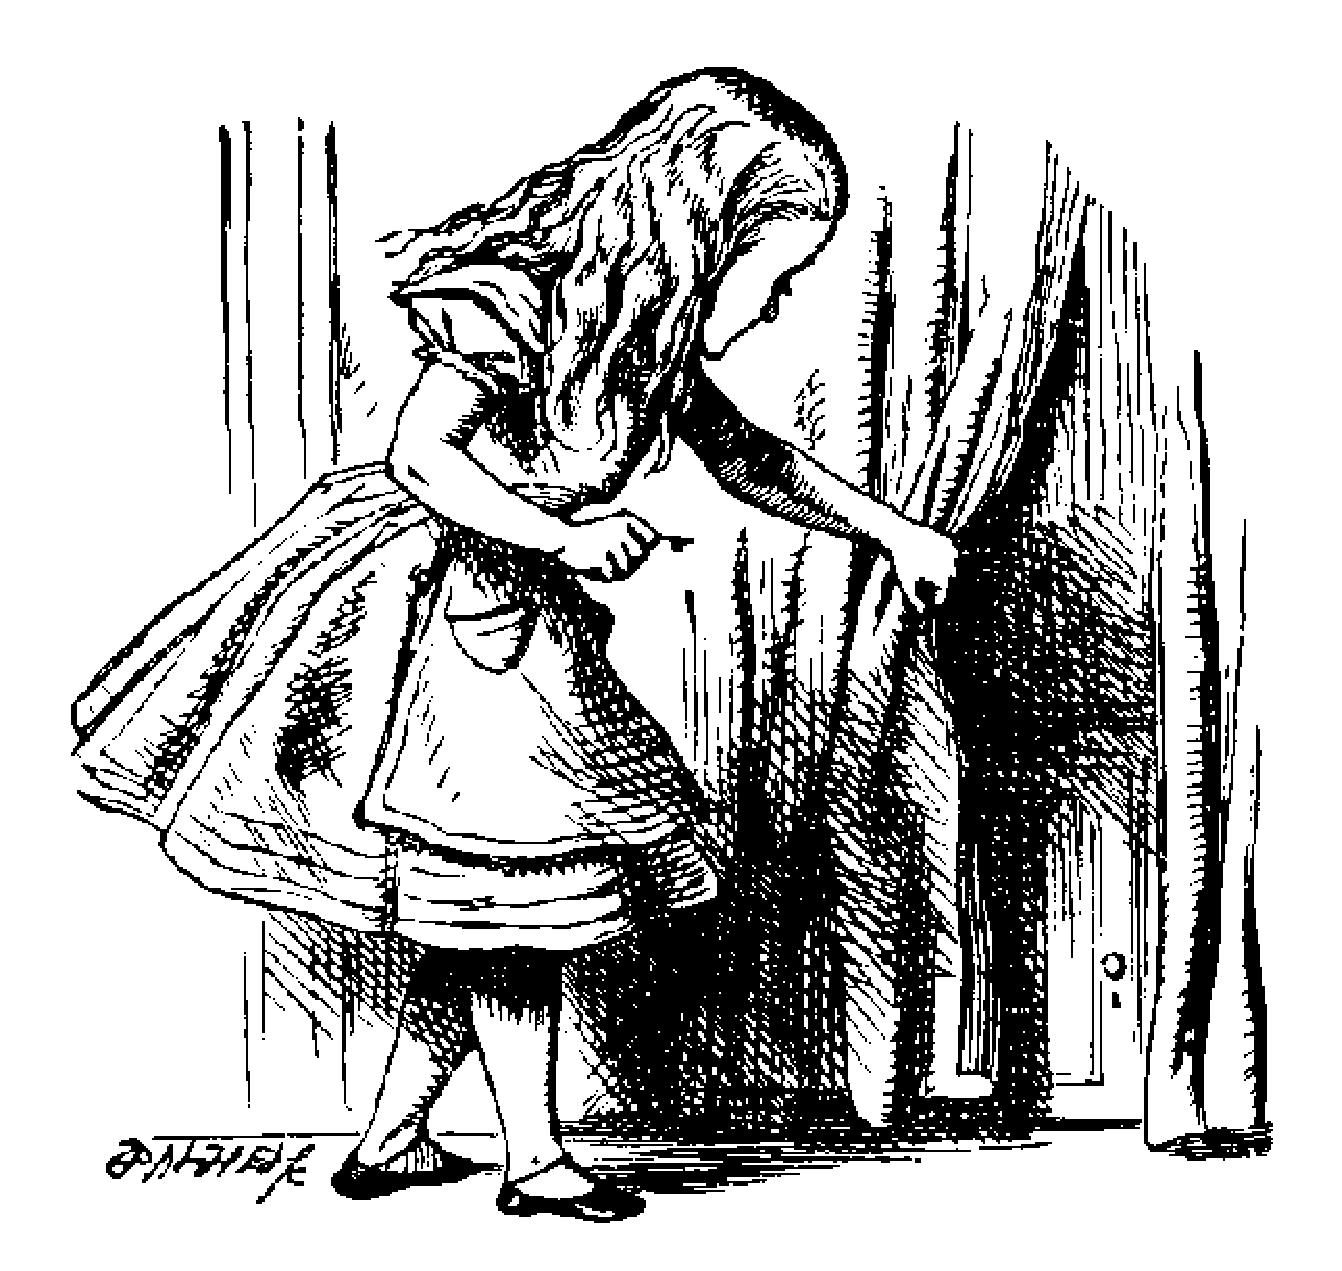
\includegraphics[width=7cm]{figures/alice}
\end{center}
\caption{Behind it was a little door}
\label{fig:alice}
\end{figure}

Alice opened the door and found that it led into a small passage, not much
larger than a rat-hole: she knelt down and looked along the passage into
the loveliest garden you ever saw.

%==============================================================================
\chapter{Design}
\label{design}

The following diagrams (especially figure \ref{fig:alice}) illustrate the
process...

%==============================================================================
\chapter{Implementation}
\label{impl}

In this chapter, we describe how the implemented the system.

%------------------------------------------------------------------------------
\section{User Interface}

Blah blah blah
Blah blah blah
Blah blah blah
Blah blah blah

% - - - - - - - - - - - - - - - - - - - - - - - - - - - - - - - - - - - - - - -
\section{Problems Encountered}
\subsection{Arthur Bigeard}
\subsection{Alexander Ferguson}
\subsection{Andrew Gibson}
\subsection{Gediminas Leikus}
\subsection{Liam Bell}

%==============================================================================
\chapter{Evaluation}

We evaluated the project by...

%==============================================================================
\chapter{Conclusion}

ASD

%==============================================================================
\section{Contributions}
\subsection{Arthur Bigeard}
\subsection{Alexander Ferguson}
\subsection{Andrew Gibson}
\subsection{Gediminas Leikus}
\subsection{Liam Bell}

%==============================================================================
\bibliographystyle{plain}
\bibliography{example}
\end{document}
